\documentclass[aspectratio=169,9pt]{beamer}
\usepackage[T5]{fontenc}
\usepackage[utf8]{inputenc}
\usepackage[vietnamese]{babel}
\usepackage{lmodern}
\usepackage{amsmath,amssymb}
\usepackage{graphicx}
\usepackage{booktabs}
\usepackage{tabularx}
\usepackage{array}
\usepackage{ragged2e}
\usepackage{tcolorbox}
\graphicspath{{assets/}}

\definecolor{PTITRed}{RGB}{166,25,31}
\definecolor{Ink}{RGB}{42,44,52}
\definecolor{Muted}{RGB}{102,108,118}
\definecolor{Line}{RGB}{188,192,200}
\definecolor{Panel}{RGB}{247,247,248}
\definecolor{PaleRed}{RGB}{249,239,240}
\definecolor{PaleGreen}{RGB}{238,246,236}

\setbeamertemplate{navigation symbols}{}
\setbeamertemplate{headline}{}
\setbeamersize{text margin left=0.55cm,text margin right=0.55cm}
\setbeamercolor{normal text}{fg=Ink,bg=white}
\setbeamercolor{frametitle}{fg=white,bg=PTITRed}
\setbeamercolor{itemize item}{fg=PTITRed}
\setbeamerfont{normal text}{size=\fontsize{8.9}{10.6}\selectfont}
\setbeamerfont{frametitle}{size=\fontsize{12.4}{14.4}\selectfont,series=\bfseries}
\setbeamerfont{itemize/enumerate body}{size=\fontsize{8.9}{10.6}\selectfont}
\setbeamertemplate{itemize item}{\raisebox{0.14ex}{\scriptsize$\blacktriangleright$}}
\setbeamertemplate{frametitle}{
  \nointerlineskip
  \begin{beamercolorbox}[wd=\paperwidth,ht=0.67cm,dp=0.36cm,center]{frametitle}
    \insertframetitle
  \end{beamercolorbox}
}
\setbeamertemplate{footline}{
  \leavevmode
  \hbox to \paperwidth{\hfill
    \colorbox{PTITRed}{\makebox[0.30cm][c]{\color{white}\fontsize{5.2}{5.2}\selectfont\insertframenumber}}
    \hspace{0.46cm}}
  \vspace{0cm}
}

\newcommand{\smallnote}[1]{{\fontsize{7.1}{8.4}\selectfont #1\par}}
\newcommand{\source}[1]{}
\newcommand{\heading}[1]{{\bfseries\color{PTITRed} #1\par}}
\newcommand{\numlabel}[1]{\colorbox{PTITRed}{\makebox[0.48cm][c]{\color{white}\bfseries #1}}}
\newcommand{\tightitems}{\setlength{\itemsep}{0.13em}\setlength{\parskip}{0pt}\setlength{\parsep}{0pt}}
\tcbset{fontupper=\RaggedRight}
\tcbset{
  panel/.style={colback=Panel,colframe=Line,boxrule=0.42pt,arc=0.8mm,left=1.6mm,right=1.6mm,top=1.1mm,bottom=1.1mm,before skip=0pt,after skip=0pt},
  keypanel/.style={colback=PaleRed,colframe=PTITRed,boxrule=0.55pt,arc=0.8mm,left=1.7mm,right=1.7mm,top=1.1mm,bottom=1.1mm,before skip=0pt,after skip=0pt},
  greenpanel/.style={colback=PaleGreen,colframe=PTITRed!45!black,boxrule=0.50pt,arc=0.8mm,left=1.7mm,right=1.7mm,top=1.1mm,bottom=1.1mm,before skip=0pt,after skip=0pt},
  titlepanel/.style={colback=white,colframe=Line,boxrule=0.45pt,arc=0mm,left=1.5mm,right=1.5mm,top=0.5mm,bottom=1.1mm,fonttitle=\bfseries,coltitle=white,colbacktitle=PTITRed,titlerule=0pt}
}
\newcolumntype{L}[1]{>{\RaggedRight\arraybackslash}p{#1}}
\newcolumntype{C}[1]{>{\Centering\arraybackslash}p{#1}}
\newcolumntype{Y}{>{\RaggedRight\arraybackslash}X}

\begin{document}

\begin{frame}
  \centering
  \vspace{-0.20cm}
  {\fontsize{10.2}{12}\selectfont Báo cáo nghiên cứu khoa học\par}
  \vspace{0.34cm}
  {\color{PTITRed}\bfseries\fontsize{12.4}{14.5}\selectfont HỌC VIỆN CÔNG NGHỆ BƯU CHÍNH VIỄN THÔNG\par}
  {\bfseries\fontsize{8.9}{10.3}\selectfont Khoa Kĩ thuật Điện tử 1\par}
  \vspace{0.23cm}
  {\color{PTITRed}\rule{0.70\paperwidth}{0.55pt}\par}
  \vspace{0.18cm}
  {\color{PTITRed}\bfseries\fontsize{15.2}{17.2}\selectfont VIDEO MAMBA\par}
  {\bfseries\fontsize{11.1}{12.9}\selectfont STATE SPACE MODEL HIỆU QUẢ\par CHO HIỂU VIDEO DÀI\par}
  \vspace{0.14cm}
  {\fontsize{8.0}{9.3}\selectfont Phân tích bài báo \textit{VideoMamba: State Space Model for Efficient Video Understanding}\par}
  \vspace{0.24cm}
  {\fontsize{7.9}{9.3}\selectfont
  \begin{tabular}{@{}l@{\hspace{0.48cm}}l@{}}
    \textcolor{PTITRed}{\bfseries Hướng nghiên cứu:} & Action Recognition trên thiết bị biên\\[0.08cm]
    \textcolor{PTITRed}{\bfseries Tác giả bài báo:} & Kunchang Li và cộng sự\\[0.08cm]
    \textcolor{PTITRed}{\bfseries Năm công bố:} & 2024\\
  \end{tabular}}\par
  \vspace{0.30cm}
  {\color{Muted}\fontsize{7.4}{8.6}\selectfont Hà Nội, tháng 08 năm 2026\par}
\end{frame}

\begin{frame}{Nội dung trình bày}
  \vspace{0.14cm}
  {\fontsize{9.3}{11.2}\selectfont
  \renewcommand{\arraystretch}{1.52}
  \begin{tabularx}{\linewidth}{@{}C{0.72cm}L{3.55cm}Y@{}}
    \numlabel{1} & \textcolor{PTITRed}{\bfseries Bài toán và mục tiêu} & Video dài tạo redundancy cục bộ, dependency toàn cục và chi phí attention lớn.\\
    \numlabel{2} & \textcolor{PTITRed}{\bfseries Kiến trúc} & Token hóa video 3D, B-Mamba và spatiotemporal scan.\\
    \numlabel{3} & \textcolor{PTITRed}{\bfseries Recipe huấn luyện} & Architecture scaling, self-distillation và masked video pretraining.\\
    \numlabel{4} & \textcolor{PTITRed}{\bfseries Thực nghiệm bài báo} & Kết quả ngắn hạn, dài hạn và hiệu năng.\\
    \numlabel{5} & \textcolor{PTITRed}{\bfseries Kết luận bài báo} & Conclusion, limitations và research relevance theo công bố gốc.\\
    \numlabel{6} & \textcolor{PTITRed}{\bfseries Thực nghiệm IPN Hand} & Fine-tuning VideoMamba trên cử chỉ tay, phân tích hội tụ và ma trận nhầm lẫn.\\
  \end{tabularx}}
  \vfill
  \source{Nguồn: VideoMamba (2024) và Thực nghiệm nhóm nghiên cứu.}
\end{frame}

\begin{frame}{1.1. Video dài cần mô hình hóa vừa cục bộ vừa toàn cục}
  \vspace{0.08cm}
  \begin{columns}[T,onlytextwidth]
    \begin{column}{0.48\textwidth}
      \begin{tcolorbox}[titlepanel,title=Hai tính chất đối nghịch,equal height group=s1_top]
        \begin{itemize}\tightitems
          \item \textbf{Redundancy cục bộ:} nhiều patch lân cận gần như trùng nhau.
          \item \textbf{Dependency toàn cục:} hành động có thể phụ thuộc vào các frame rất xa.
          \item \textbf{Mục tiêu:} đồng thời nhận biết motion tinh vi và ngữ cảnh dài.
        \end{itemize}
      \end{tcolorbox}
      \vspace{0.14cm}
      \begin{tcolorbox}[panel,equal height group=s1_bot]
        \heading{Chi phí theo độ dài chuỗi $L$}
        \vspace{-0.12cm}
        \[
          \begin{array}{c}
            \text{Self-Attention}:\ O(L^2D)\\[-0.1ex]
            \text{Selective SSM}:\ O(LD)
          \end{array}
        \]
        \smallnote{Khi tăng frame hoặc resolution, $L$ tăng nhanh; quadratic attention trở thành nút thắt memory.}
      \end{tcolorbox}
    \end{column}
    \begin{column}{0.48\textwidth}
      \begin{tcolorbox}[titlepanel,title=Khoảng trống của các họ mô hình,equal height group=s1_top]
        \renewcommand{\arraystretch}{1.28}
        {\fontsize{7.4}{8.5}\selectfont\begin{tabularx}{\linewidth}{@{}L{1.72cm}Y Y@{}}
          \toprule
          \textbf{Họ} & \textbf{Điểm mạnh} & \textbf{Hạn chế chính}\\
          \midrule
          3D CNN & Receptive field cục bộ & Khó giữ dependency dài.\\
          Transformer & Context toàn cục & Attention đắt với video dài.\\
          VideoMamba & Scan tuyến tính & Cần thiết kế scan phù hợp.\\
          \bottomrule
        \end{tabularx}}
      \end{tcolorbox}
      \vspace{0.14cm}
      \begin{tcolorbox}[keypanel,equal height group=s1_bot]
        \heading{Mục tiêu nghiên cứu}
        Điều chỉnh Mamba cho video nhằm mô hình hóa dependency không-thời gian dài với chi phí tuyến tính theo số token.
      \end{tcolorbox}
    \end{column}
  \end{columns}
  \vfill
  \source{Nguồn: VideoMamba, Introduction; độ phức tạp SSM theo Section 3.1.}
\end{frame}

\begin{frame}{2.1. Input video được chuyển thành chuỗi token không-thời gian}
  \vspace{0.10cm}
  \begin{columns}[T,onlytextwidth]
    \begin{column}{0.30\textwidth}
      \begin{tcolorbox}[titlepanel,title=1. Video tensor $\mathbf X_v$, equal height group=s2]
        \centering
        \[
          \mathbf X_v\in\mathbb R^{3\times T\times H\times W}
        \]
        \vspace{-0.12cm}
        \raggedright
        $\mathbf X_v$: video clip input, đã lấy mẫu frame và resize/crop.\par
        \vspace{0.08cm}
        {\fontsize{7.35}{8.55}\selectfont
        \textbf{3}: ba kênh màu RGB.\par
        \textbf{$T$}: số frame theo trục thời gian.\par
        \textbf{$H,W$}: chiều cao, chiều rộng của mỗi frame.}
      \end{tcolorbox}
    \end{column}
    \begin{column}{0.33\textwidth}
      \begin{tcolorbox}[titlepanel,title=2. Patchify và $L$, equal height group=s2]
        \raggedright
        \textbf{Kernel = stride:} $(1\times16\times16)$.\\
        Mỗi patch nằm trong một frame, nên $t=T$.\par
        \vspace{0.08cm}
        Lưới patch mỗi frame:
        \centering
        \[
          h=H/16,\qquad w=W/16
        \]
        \[
          L=T\times\frac{H}{16}\times\frac{W}{16}
        \]
        \raggedright
        \textbf{$L$}: số patch token.
      \end{tcolorbox}
    \end{column}
    \begin{column}{0.30\textwidth}
      \begin{tcolorbox}[titlepanel,title=3. Chuỗi đưa vào encoder, equal height group=s2]
        \centering
        {\fontsize{7.0}{8.25}\selectfont
        \[
          \begin{aligned}
            \mathbf X&=[\mathbf X_{cls},\mathbf X_p]\\[-0.04cm]
                     &+\mathbf p_s+\mathbf p_t
          \end{aligned}
        \]
        \raggedright
        $\mathbf X_p$: $L$ patch embedding, mỗi token $C$ chiều.\par
        \textbf{[CLS]}: token học được; đại diện toàn video, đi vào classification head.\par
        $\mathbf p_s$: vị trí patch trong frame.\par
        $\mathbf p_t$: thời điểm/frame của patch.}
      \end{tcolorbox}
    \end{column}
  \end{columns}
\end{frame}

\begin{frame}{2.2. VideoMamba: encoder ViT-like với B-Mamba cho chuỗi token 3D}
  \vspace{0.04cm}
  \centering
  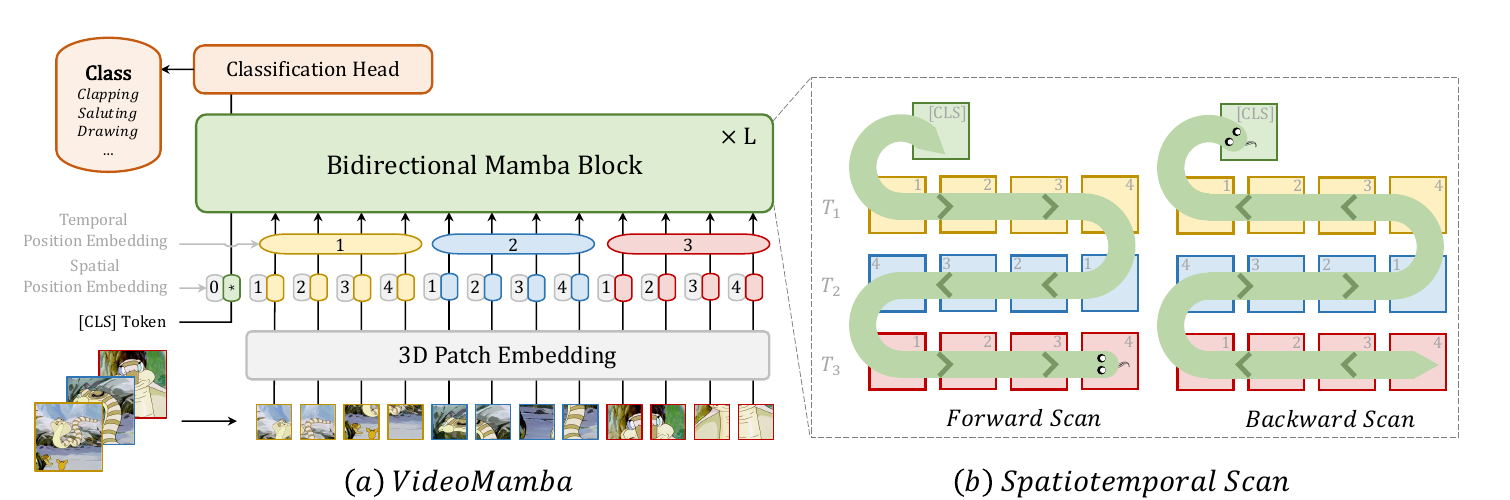
\includegraphics[width=0.97\linewidth,height=3.65cm,keepaspectratio]{figure-3-framework.png}\par
  \vspace{-0.02cm}
  \begin{columns}[T,onlytextwidth]
    \begin{column}{0.58\textwidth}
      \begin{tcolorbox}[titlepanel,title=Luồng dữ liệu VideoMamba,equal height group=s3_bot]
        {\fontsize{7.5}{8.7}\selectfont
        \renewcommand{\arraystretch}{1.18}
        \begin{tabularx}{\linewidth}{@{}C{0.70cm}Y@{}}
          \numlabel{1} & 3D convolution $(1\times16\times16)$ tạo các patch không-thời gian không chồng lấp.\\
          \numlabel{2} & Ghép [CLS] với patch sequence; cộng spatial và temporal position embedding.\\
          \numlabel{3} & Xếp chồng $L$ B-Mamba block; biểu diễn [CLS] đi qua linear head.\\
        \end{tabularx}}
      \end{tcolorbox}
    \end{column}
    \begin{column}{0.38\textwidth}
      \begin{tcolorbox}[keypanel,equal height group=s3_bot]
        \heading{Video tạo chuỗi token dài}
        {\fontsize{7.4}{8.5}\selectfont
        \[\mathbf X_v\in\mathbb R^{3\times T\times H\times W}\]
        \[L=\frac{T}{1}\cdot\frac{H}{16}\cdot\frac{W}{16}\]
        Ví dụ $16\times224\times224\Rightarrow16\times14\times14=3136$ token.}
      \end{tcolorbox}
    \end{column}
  \end{columns}
  \vfill
  \source{Nguồn: VideoMamba, Hình 3 và Section 3.2.}
\end{frame}

\begin{frame}{2.3. Spatiotemporal bidirectional scan strategies}
  \vspace{0.06cm}
  \centering
  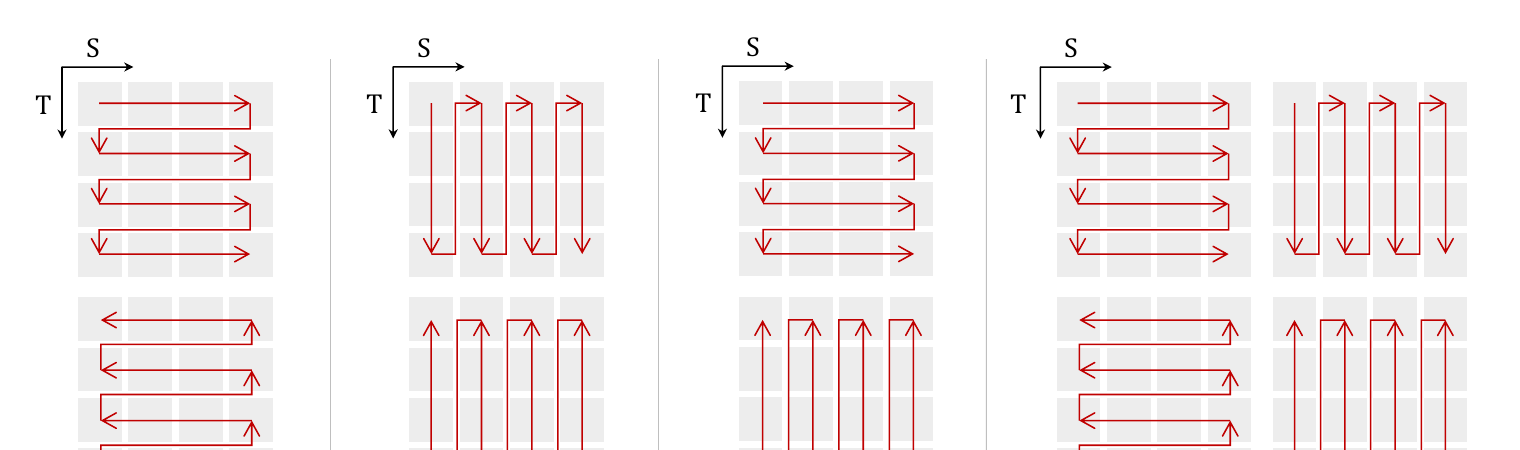
\includegraphics[width=0.98\linewidth,height=3.75cm,keepaspectratio]{figure-4-scan.png}\par
  \vspace{-0.02cm}
  \begin{columns}[T,onlytextwidth]
    \begin{column}{0.48\textwidth}
      \begin{tcolorbox}[panel,equal height group=s4_bot]
        \heading{Điểm khác nhau}
        Spatial-first, temporal-first, spatiotemporal v1 và v2 đều chạy forward + backward; khác biệt duy nhất là thứ tự token trước khi đi vào SSM.
      \end{tcolorbox}
    \end{column}
    \begin{column}{0.48\textwidth}
      \begin{tcolorbox}[keypanel,equal height group=s4_bot]
        \heading{Kết quả ablation}
        Trên SSV2, spatial-first đạt 65.1\%, cao nhất trong các scan strategy được đánh giá; tác giả chọn thiết kế này vì đơn giản.
      \end{tcolorbox}
    \end{column}
  \end{columns}
  \vfill
  \source{Nguồn: VideoMamba, Hình 4, Hình 7 và Section 3.2.}
\end{frame}

\begin{frame}{3.1. Masked video pretraining: objective và masking strategy}
  \vspace{0.04cm}
  \centering
  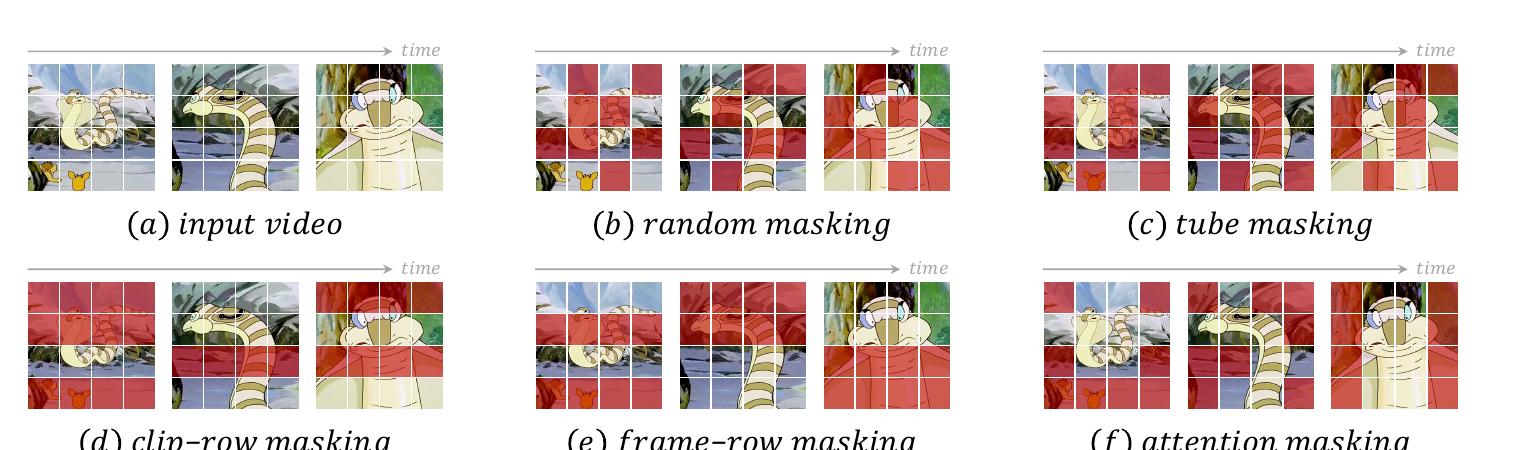
\includegraphics[width=0.97\linewidth,height=3.20cm,keepaspectratio]{figure-5-masking.png}\par
  \vspace{0.04cm}
  \begin{columns}[T,onlytextwidth]
    \begin{column}{0.54\textwidth}
      \begin{tcolorbox}[panel,equal height group=s5_bot]
        \heading{Objective}
        VideoMamba được pretrain trên video; output của token không bị mask được align với feature từ CLIP-ViT teacher. Masking strategy là một thành phần của recipe này.
      \end{tcolorbox}
    \end{column}
    \begin{column}{0.42\textwidth}
      \begin{tcolorbox}[keypanel,equal height group=s5_bot]
        \heading{Masking và ablation trên SSV2}
        \smallnote{Conv1D ưu tiên token liên tục. Random: 67.4\quad Tube: 66.3\\ Clip-row: 68.2\quad Frame-row: 67.8\quad \textbf{Attention: 68.5}}
      \end{tcolorbox}
    \end{column}
  \end{columns}
  \vfill
  \source{Nguồn: VideoMamba, Hình 5, Table 5 và Section 3.4.}
\end{frame}

\begin{frame}{3.2. Architecture scaling và self-distillation}
  \vspace{0.04cm}
  \begin{columns}[T,onlytextwidth]
    \begin{column}{0.31\textwidth}
      \begin{tcolorbox}[titlepanel,title=Model scale,height=2.65cm]
        {\fontsize{7.2}{8.2}\selectfont
        \renewcommand{\arraystretch}{1.18}
        \begin{tabularx}{\linewidth}{@{}Y C{0.62cm} C{0.62cm} C{0.62cm}@{}}
          \toprule
          \textbf{Model} & \textbf{D} & \textbf{Dim} & \textbf{P}\\
          \midrule
          Tiny & 24 & 192 & 7M\\
          Small & 24 & 384 & 26M\\
          Middle & 32 & 576 & 74M\\
          Base & 24 & 768 & 98M\\
          \bottomrule
        \end{tabularx}}
      \end{tcolorbox}
    \end{column}
    \begin{column}{0.65\textwidth}
      \centering
      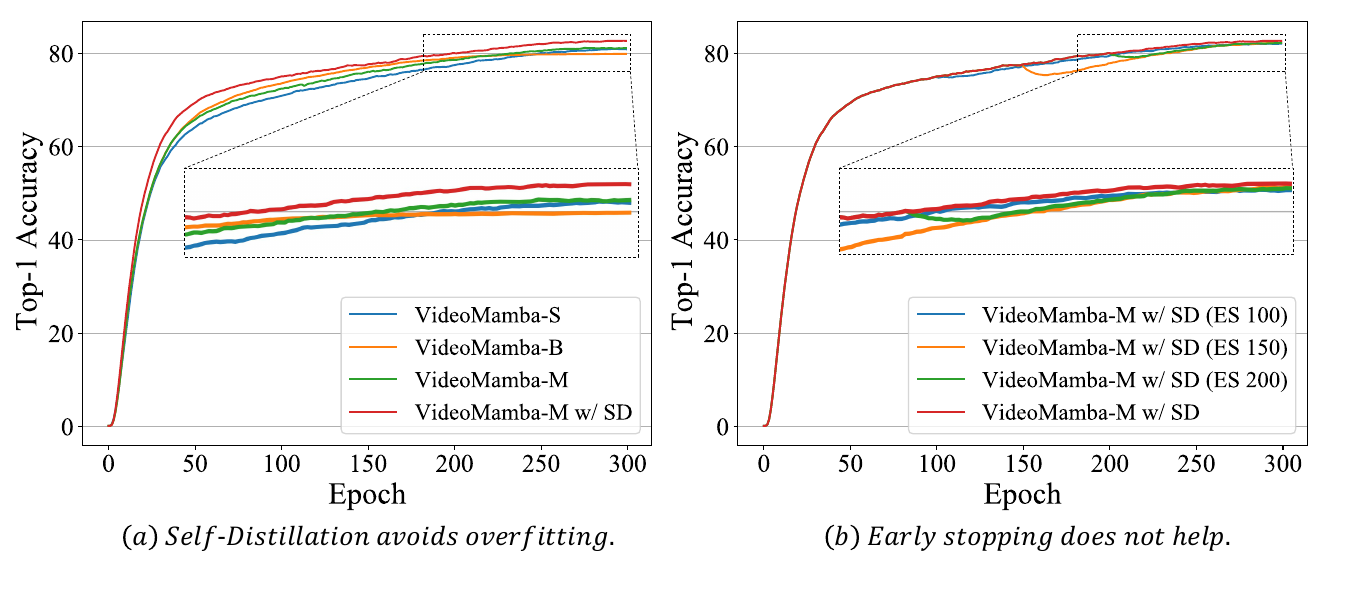
\includegraphics[width=\linewidth,height=2.65cm,keepaspectratio]{figure-6-distillation.png}\par
    \end{column}
  \end{columns}
  \vspace{0.04cm}
  \begin{columns}[T,onlytextwidth]
    \begin{column}{0.48\textwidth}
      \begin{tcolorbox}[panel,equal height group=s6_bot]
        \heading{Quan sát khi scale}
        VideoMamba-B huấn luyện từ đầu có xu hướng overfit và không tốt hơn VideoMamba-S; early stopping không thay thế được regularization.
      \end{tcolorbox}
    \end{column}
    \begin{column}{0.48\textwidth}
      \begin{tcolorbox}[keypanel,equal height group=s6_bot]
        \heading{Teacher $\rightarrow$ student, chỉ khi train}
        VideoMamba-S đã học tốt làm teacher cho VideoMamba-M; căn chỉnh final feature map bằng L2 loss. Inference vẫn là một VideoMamba duy nhất.
      \end{tcolorbox}
    \end{column}
  \end{columns}
  \vfill
  \source{Nguồn: VideoMamba, Table 1, Hình 6 và Sections 3.3, 4.1.}
\end{frame}

\begin{frame}{4.1. Thiết lập thực nghiệm}
  \vspace{0.10cm}
  \begin{columns}[T,onlytextwidth]
    \begin{column}{0.48\textwidth}
      \begin{tcolorbox}[titlepanel,title=Scale up trên ảnh,equal height group=s7_top]
        \heading{ImageNet-1K}
        \smallnote{Kiểm tra khả năng scale model/input trước khi transfer sang video; benchmark có 1.28M ảnh train, 1,000 lớp.}
      \end{tcolorbox}
      \vspace{0.14cm}
      \begin{tcolorbox}[titlepanel,title=Video ngắn,equal height group=s7_bot]
        \heading{Kinetics-400}
        \smallnote{Phân loại hành động theo scene; video trung bình 10 giây.}
        \vspace{0.08cm}
        \heading{Something-Something V2}
        \smallnote{Nhạy với diễn biến thời gian; video trung bình 4 giây.}
      \end{tcolorbox}
    \end{column}
    \begin{column}{0.48\textwidth}
      \begin{tcolorbox}[greenpanel,equal height group=s7_top]
        \heading{Thiết lập chính}
        Fine-tune video từ ImageNet-1K; masked alignment dùng CLIP-ViT teacher cho pretraining self-supervised.
      \end{tcolorbox}
      \vspace{0.14cm}
      \begin{tcolorbox}[titlepanel,title=Video dài,equal height group=s7_bot]
        \heading{Breakfast và COIN}
        \smallnote{Nhận biết hoạt động và thủ tục dài; Breakfast gồm 77 giờ video, COIN có 180 procedural tasks.}
        \vspace{0.08cm}
        \heading{LVU}
        \smallnote{Long-form Video Understanding: clip phim 1--3 phút, 9 tác vụ content, metadata và user engagement.}
      \end{tcolorbox}
    \end{column}
  \end{columns}
  \vfill
  \source{Nguồn: VideoMamba, Sections 4.1--4.4.}
\end{frame}

\begin{frame}{4.2. Kết quả video ngắn: Kinetics-400 và Something-Something V2}
  \vspace{0.08cm}
  \begin{columns}[T,onlytextwidth]
    \begin{column}{0.48\textwidth}
      \begin{tcolorbox}[titlepanel,title={Kinetics-400, supervised},equal height group=s8_top]
        {\fontsize{7.9}{9.0}\selectfont
        \renewcommand{\arraystretch}{1.24}
        \begin{tabularx}{\linewidth}{@{}Y C{1.05cm} C{1.05cm}@{}}
          \toprule
          \textbf{Model} & \textbf{Top-1} & \textbf{Top-5}\\
          \midrule
          TimeSformer-L & 80.7 & 94.7\\
          ViViT-L & 81.3 & 95.4\\
          \textbf{VideoMamba-M$_{f64}$} & \textbf{83.3} & \textbf{96.1}\\
          \bottomrule
        \end{tabularx}}
      \end{tcolorbox}
      \vspace{0.14cm}
      \begin{tcolorbox}[panel,equal height group=s8_bot]
        \heading{Ablation: scan strategy}
        Spatial-first đạt 65.1\% trên SSV2, cao nhất trong các scan strategy được đánh giá; Alternative SF\&TF đạt cùng mức nhưng phức tạp hơn.
      \end{tcolorbox}
    \end{column}
    \begin{column}{0.48\textwidth}
      \begin{tcolorbox}[titlepanel,title={Something-Something V2, supervised},equal height group=s8_top]
        {\fontsize{7.9}{9.0}\selectfont
        \renewcommand{\arraystretch}{1.24}
        \begin{tabularx}{\linewidth}{@{}Y C{1.05cm} C{1.05cm}@{}}
          \toprule
          \textbf{Model} & \textbf{Top-1} & \textbf{Top-5}\\
          \midrule
          TimeSformer-L & 62.5 & --\\
          ViViT-L & 65.4 & 89.8\\
          \textbf{VideoMamba-M} & \textbf{68.4} & \textbf{91.6}\\
          \bottomrule
        \end{tabularx}}
      \end{tcolorbox}
      \vspace{0.14cm}
      \begin{tcolorbox}[keypanel,equal height group=s8_bot]
        \heading{Ablation: token budget}
        K400 tăng theo số frame; SSV2 có optimum khác vì video ngắn. Nhiều token hơn không luôn cải thiện kết quả.
      \end{tcolorbox}
    \end{column}
  \end{columns}
  \vfill
  \source{Nguồn: VideoMamba, Tables 3--4, Hình 7.}
\end{frame}

\begin{frame}{4.3. Kết quả video dài: Breakfast, COIN và LVU}
  \vspace{0.10cm}
  \begin{columns}[T,onlytextwidth]
    \begin{column}{0.56\textwidth}
      \begin{tcolorbox}[titlepanel,title=Kết quả long-term video understanding,height=4.65cm]
        {\fontsize{8.1}{9.2}\selectfont
        \renewcommand{\arraystretch}{1.37}
        \begin{tabularx}{\linewidth}{@{}L{1.55cm}Y C{1.25cm} C{1.25cm}@{}}
          \toprule
          \textbf{Benchmark} & \textbf{Cấu hình} & \textbf{Metric} & \textbf{Kết quả}\\
          \midrule
          Breakfast & VideoMamba$_{f32}$ & Top-1 & \textbf{97.9}\\
          COIN & VideoMamba$_{f64}$ & Top-1 & \textbf{90.4}\\
          LVU & VideoMamba$_{f32}$ & Scene & \textbf{70.37}\\
          LVU & VideoMamba$_{f32}$ & Director & \textbf{67.29}\\
          LVU & VideoMamba$_{f32}$ & Genre & \textbf{65.24}\\
          \bottomrule
        \end{tabularx}}
      \end{tcolorbox}
    \end{column}
    \begin{column}{0.40\textwidth}
      \begin{tcolorbox}[panel,height=2.70cm]
        \heading{Điểm khác biệt}
        \begin{itemize}\tightitems
          \item Train end-to-end trên video dài.
          \item Không phụ thuộc pipeline trích feature trước rồi mới suy luận.
          \item Dễ tăng frame nhờ scan có chi phí tuyến tính.
        \end{itemize}
      \end{tcolorbox}
      \vspace{0.14cm}
      \begin{tcolorbox}[keypanel,height=1.81cm]
        \heading{Thông điệp}
        Với long context, cách token mixer ảnh hưởng trực tiếp cả memory lẫn khả năng học quan hệ xa.
      \end{tcolorbox}
    \end{column}
  \end{columns}
  \vfill
  \source{Nguồn: VideoMamba, Tables 6--7 và Section 4.3.}
\end{frame}

\begin{frame}{4.4. Computational efficiency trên video dài}
  \vspace{0.08cm}
  \centering
  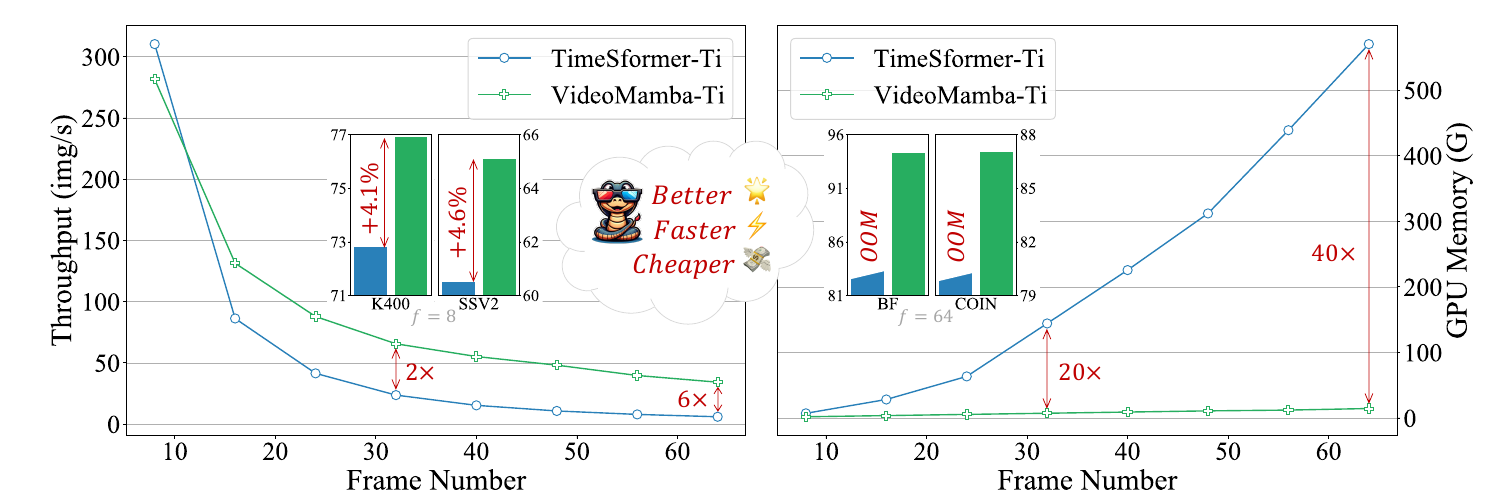
\includegraphics[width=0.96\linewidth,height=3.65cm,keepaspectratio]{figure-1-performance.png}\par
  \vspace{0.04cm}
  \begin{columns}[T,onlytextwidth]
    \begin{column}{0.48\textwidth}
      \begin{tcolorbox}[greenpanel,equal height group=s9_bot]
        \heading{Throughput}
        32 frame: xấp xỉ \textbf{2$\times$} nhanh hơn TimeSformer-Ti.\\
        64 frame: xấp xỉ \textbf{6$\times$} nhanh hơn.
      \end{tcolorbox}
    \end{column}
    \begin{column}{0.48\textwidth}
      \begin{tcolorbox}[keypanel,equal height group=s9_bot]
        \heading{GPU memory}
        32 frame: dùng khoảng \textbf{20$\times$} ít memory hơn.\\
        64 frame: dùng khoảng \textbf{40$\times$} ít memory hơn.
      \end{tcolorbox}
    \end{column}
  \end{columns}
  \vfill
  \source{Nguồn: VideoMamba, Hình 1; so sánh VideoMamba-Ti với TimeSformer-Ti trên cấu hình paper.}
\end{frame}

\begin{frame}{5. Conclusion, limitations và research relevance}
  \vspace{0.08cm}
  \begin{columns}[T,onlytextwidth]
    \begin{column}{0.48\textwidth}
      \begin{tcolorbox}[titlepanel,title=Kết luận của bài báo,equal height group=s5_top]
        \begin{itemize}\tightitems
          \item \textbf{Scale:} self-distillation giúp model lớn hội tụ tốt hơn.
          \item \textbf{Motion:} spatial-first scan và masking giữ nhạy với hành động ngắn.
          \item \textbf{Long video:} train end-to-end hiệu quả hơn các pipeline feature-based.
          \item \textbf{Multimodal:} có thể kết hợp text encoder và cross-modal decoder.
        \end{itemize}
      \end{tcolorbox}
      \vspace{0.14cm}
      \begin{tcolorbox}[keypanel,equal height group=s5_bot]
        \heading{Relevance to our research}
        \smallnote{Diễn giải cho Action Recognition Edge: linear scan có thể hỗ trợ tăng số frame trong memory giới hạn. Latency thực tế cần benchmark trên đúng Jetson/NPU và pipeline decode.}
      \end{tcolorbox}
    \end{column}
    \begin{column}{0.48\textwidth}
      \begin{tcolorbox}[titlepanel,title=Giới hạn được tác giả nêu,equal height group=s5_top]
        \begin{itemize}\tightitems
          \item Chưa kiểm chứng toàn diện ở kích thước cực lớn.
          \item Chưa tích hợp audio hoặc mô hình ngôn ngữ lớn cho video theo giờ.
          \item Chưa đánh giá trực tiếp khi chuyển từ benchmark GPU sang thiết bị edge.
        \end{itemize}
      \end{tcolorbox}
      \vspace{0.14cm}
      \begin{tcolorbox}[greenpanel,equal height group=s5_bot]
        \heading{Phạm vi kết luận}
        \smallnote{Các kết quả hiệu năng và accuracy được báo cáo theo cấu hình training, input và GPU của paper; không suy diễn trực tiếp sang một edge platform cụ thể.}
      \end{tcolorbox}
    \end{column}
  \end{columns}
  \vfill
  \source{Nguồn: VideoMamba, Abstract, Sections 4.4--5.}
\end{frame}

\begin{frame}{6.1. Thực nghiệm Fine-tuning VideoMamba trên IPN Hand}
  \vspace{0.02cm}
  \begin{columns}[T,onlytextwidth]
    \begin{column}{0.48\textwidth}
      \begin{tcolorbox}[titlepanel,title=Tập dữ liệu IPN Hand (Subject-wise),equal height group=s6_1]
        {\fontsize{7.4}{8.7}\selectfont
        \begin{itemize}\tightitems
          \item \textbf{Tác vụ:} Nhận dạng 14 lớp cử chỉ tay tương tác vô chạm.
          \item \textbf{Quy mô:} 200 video AVI, 5,649 gesture instances.
          \item \textbf{Subject-wise split (chia theo người quay):}
            \begin{itemize}\tightitems
              \item \textit{Train:} 20 subjects (140 video, 3,969 mẫu)
              \item \textit{Val:} 6 subjects (36 video, 1,058 mẫu)
              \item \textit{Test:} 3 subjects (24 video, 622 mẫu)
            \end{itemize}
          \item \textbf{Data Pipeline:} Đọc trực tiếp $[t_{\text{start}}, t_{\text{end}}]$ qua Decord, không sinh video clip vật lý phụ.
          \item \textbf{Đầu vào mô hình:} 16 frames uniform sampling, $224\times 224$, Random Resized Crop + Color Jitter.
        \end{itemize}}
      \end{tcolorbox}
    \end{column}
    \begin{column}{0.48\textwidth}
      \begin{tcolorbox}[titlepanel,title=Cấu hình Huấn luyện chi tiết (Recipe),equal height group=s6_1]
        {\fontsize{7.1}{8.2}\selectfont
        \renewcommand{\arraystretch}{1.08}
        \begin{tabularx}{\linewidth}{@{}L{2.55cm}Y@{}}
          \toprule
          \textbf{Tham số} & \textbf{Thiết lập thực nghiệm}\\
          \midrule
          Backbone & \textbf{VideoMamba-Tiny} (7M params)\\
          Khởi tạo & ImageNet-1K pretrained weights\\
          Phần cứng & $2\times$ NVIDIA Tesla T4 (FP32 DDP)\\
          Effective Batch & 16 (8 clips / GPU)\\
          Optimizer & AdamW ($\beta_1=0.9, \beta_2=0.999$, $\text{wd}=0.05$)\\
          Learning Rate & Base $\text{LR}=1\times 10^{-4}$ (Cosine decay)\\
          Warmup & 2,480 steps khởi động\\
          Số Epochs & 30 epochs ($\approx$ 8h 07m tổng thời gian)\\
          Loss Function & CrossEntropyLoss (FP32 save/resume)\\
          \bottomrule
        \end{tabularx}}
        \vspace{0.03cm}
        \smallnote{\textbf{Tối ưu:} Cached wheels \texttt{causal\_conv1d} \& \texttt{mamba\_ssm} cho T4.}
      \end{tcolorbox}
    \end{column}
  \end{columns}
  \vfill
  \source{Thực nghiệm nhóm: Huấn luyện trên Kaggle $2\times$ T4 GPU, dataset IPN Hand.}
\end{frame}

\begin{frame}{6.2. Quá trình huấn luyện và đồ thị hội tụ}
  \vspace{-0.15cm}
  \centering
  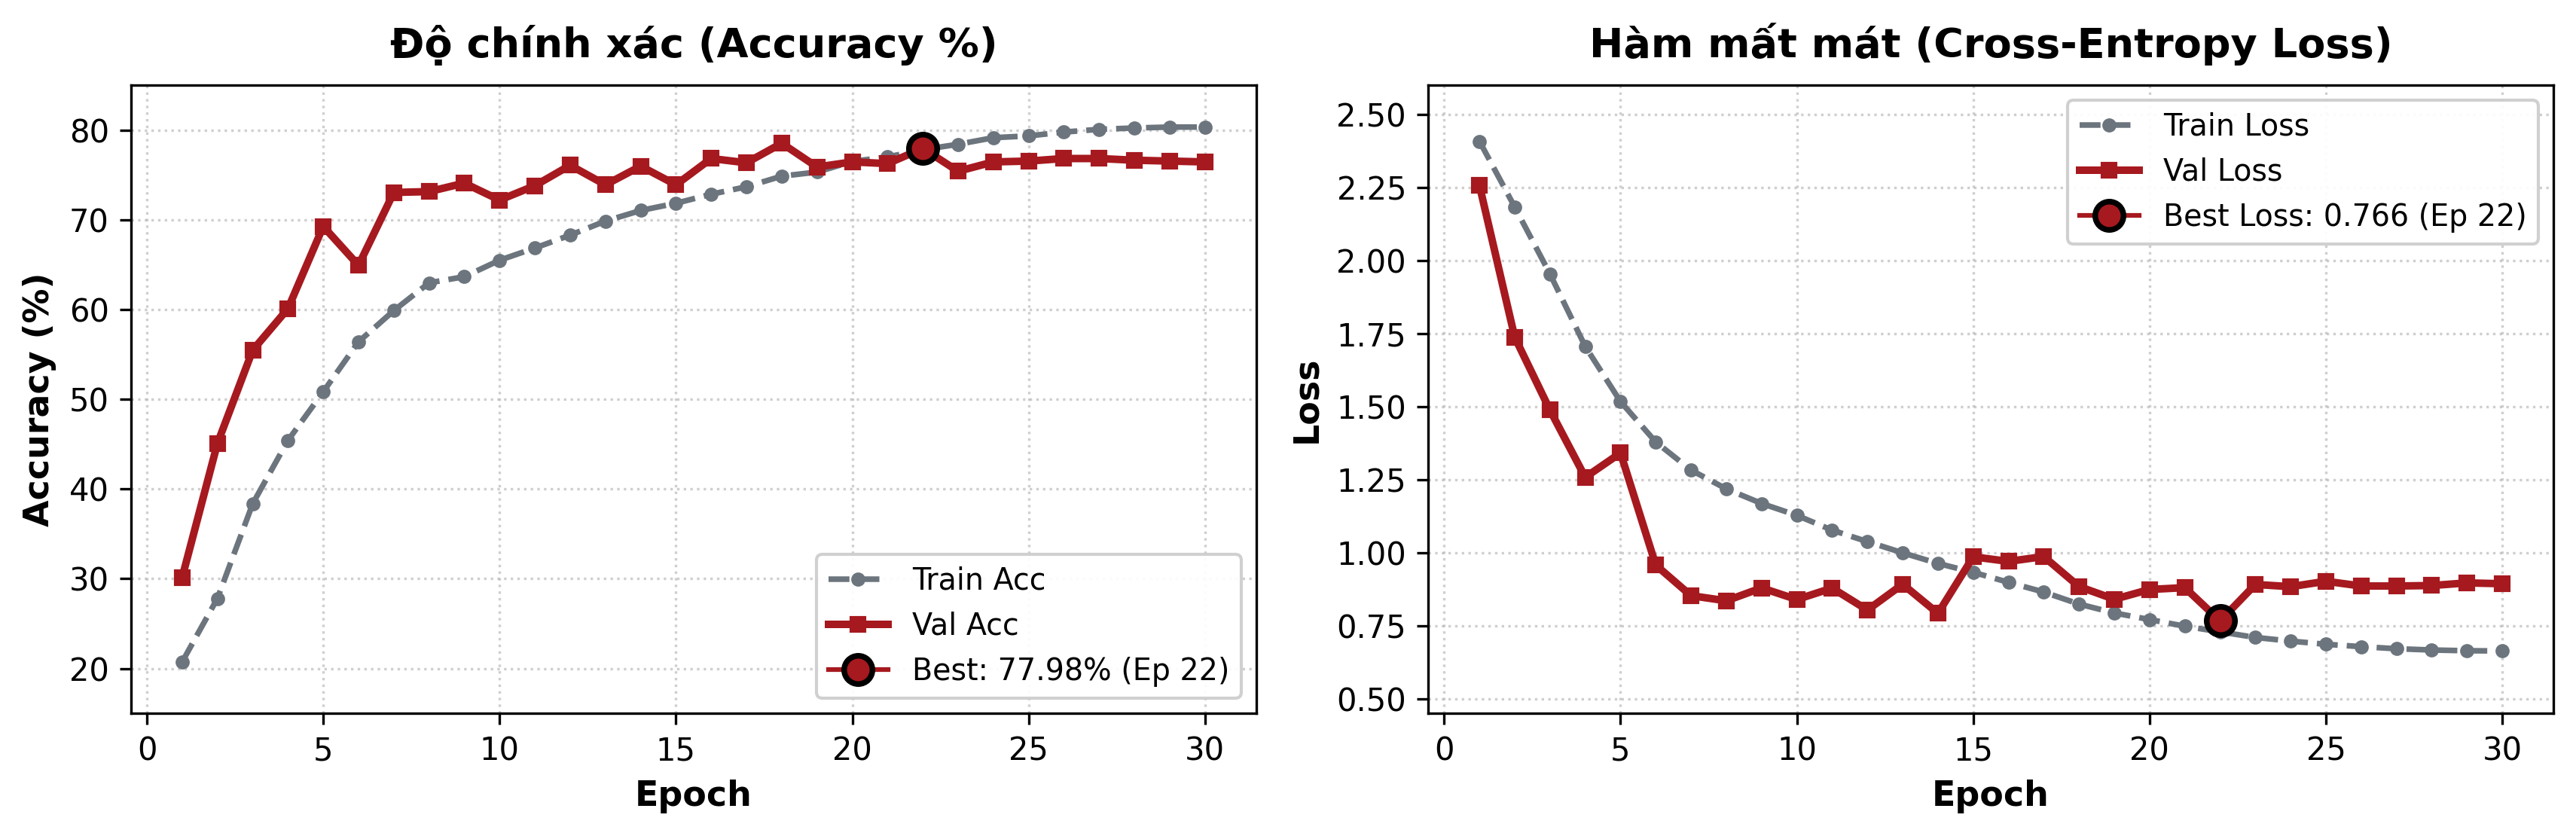
\includegraphics[width=0.98\linewidth,height=2.68cm,keepaspectratio]{ipn_curves_slide.png}\par
  \vspace{0.02cm}
  \begin{columns}[T,onlytextwidth]
    \begin{column}{0.48\textwidth}
      \begin{tcolorbox}[titlepanel,title=Đặc điểm hội tụ qua 30 Epochs,equal height group=s6_2]
        {\fontsize{7.2}{8.4}\selectfont
        \begin{itemize}\tightitems
          \item \textbf{Khởi động nhanh:} Chuyển giao hiệu quả từ ImageNet-1K; Val Acc đạt 73.1\% ngay từ Epoch 7.
          \item \textbf{Điểm tối ưu:} Đạt \textbf{Val Acc cao nhất = 77.98\%} tại \textbf{Epoch 22} (Val Loss đạt 0.7664).
          \item \textbf{Checkpoint:} \texttt{checkpoint-best.pth} kích thước gọn nhẹ (\textbf{80.15 MB}), sẵn sàng deploy.
        \end{itemize}}
      \end{tcolorbox}
    \end{column}
    \begin{column}{0.48\textwidth}
      \begin{tcolorbox}[titlepanel,title=Tính ổn định của VideoMamba,equal height group=s6_2]
        {\fontsize{7.2}{8.4}\selectfont
        \begin{itemize}\tightitems
          \item Đường cong Loss và Acc mượt mà, không gặp hiện tượng tràn số (NaN / Inf) hay sụp đổ gradient.
          \item Cơ chế Cosine LR decay giúp mô hình tinh chỉnh trọng số ổn định trong 10 epoch cuối.
          \item Thời gian trung bình mỗi epoch $\approx 16$ phút trên $2\times$ T4.
        \end{itemize}}
      \end{tcolorbox}
    \end{column}
  \end{columns}
  \vfill
  \source{Nguồn: Nhật ký huấn luyện \texttt{log.txt}, 30 epochs trên IPN Hand.}
\end{frame}

\begin{frame}{6.3. Đánh giá hiệu năng kiểm thử trên tập Test}
  \vspace{0.08cm}
  \begin{columns}[T,onlytextwidth]
    \begin{column}{0.48\textwidth}
      \begin{tcolorbox}[titlepanel,title=Hiệu năng tổng thể Test Set (622 mẫu),equal height group=s6_3_top]
        {\fontsize{7.4}{8.6}\selectfont
        \renewcommand{\arraystretch}{1.20}
        \begin{tabularx}{\linewidth}{@{}L{2.85cm}C{1.35cm}Y@{}}
          \toprule
          \textbf{Giao thức} & \textbf{Top-1} & \textbf{Chi tiết}\\
          \midrule
          Multi-view (12 views) & \textbf{81.83\%} & Top-5: 96.62\%\\
          Single-view (Center) & \textbf{77.97\%} & Balanced: 68.03\%\\
          \bottomrule
        \end{tabularx}}
        \vspace{0.06cm}
        \smallnote{\textbf{Weighted F1 = 77.38\%} \quad|\quad \textbf{Macro F1 = 68.39\%}}
      \end{tcolorbox}
      \vspace{0.14cm}
      \begin{tcolorbox}[panel,equal height group=s6_3_bot]
        \heading{Khả năng tổng quát hóa}
        \smallnote{Mô hình kiểm thử trên 3 đối tượng (Subjects 1, 10, 17) hoàn toàn mới, chứng minh khả năng thích ứng tốt với người dùng khác nhau.}
      \end{tcolorbox}
    \end{column}
    \begin{column}{0.48\textwidth}
      \begin{tcolorbox}[titlepanel,title=Phân tích theo nhóm cử chỉ tay,equal height group=s6_3_top]
        {\fontsize{7.3}{8.5}\selectfont
        \begin{itemize}\tightitems
          \item \textbf{Cử chỉ giữ ngón / tĩnh (D0X, B0A, B0B):} F1 rất cao (\textbf{87.2\% -- 88.8\%}).
          \item \textbf{Cử chỉ vuốt/ném (G03--G06):} F1 đạt \textbf{72.3\% -- 85.7\%} (G05 Throw left đạt Precision 100\%).
          \item \textbf{Cử chỉ click vi mô (G01, G02):} F1 thấp hơn do thời lượng ngắn, dễ nhầm giữa 1 và 2 ngón trong video độ phân giải thường.
        \end{itemize}}
      \end{tcolorbox}
      \vspace{0.14cm}
      \begin{tcolorbox}[greenpanel,equal height group=s6_3_bot]
        \heading{Ưu thế Spatiotemporal Scan}
        \smallnote{Mô hình hóa hoàn hảo các chuyển động định hướng không gian lớn (Throw, Zoom) nhờ cơ chế quét hai chiều liên tục.}
      \end{tcolorbox}
    \end{column}
  \end{columns}
  \vfill
  \source{Đánh giá độc lập trên tập Test (24 raw videos, 3 đối tượng chưa từng xuất hiện trong tập Train/Val).}
\end{frame}

\begin{frame}{6.4. Ma trận nhầm lẫn chi tiết (Normalized Confusion Matrix)}
  \vspace{-0.18cm}
  \begin{columns}[T,onlytextwidth]
    \begin{column}{0.66\textwidth}
      \centering
      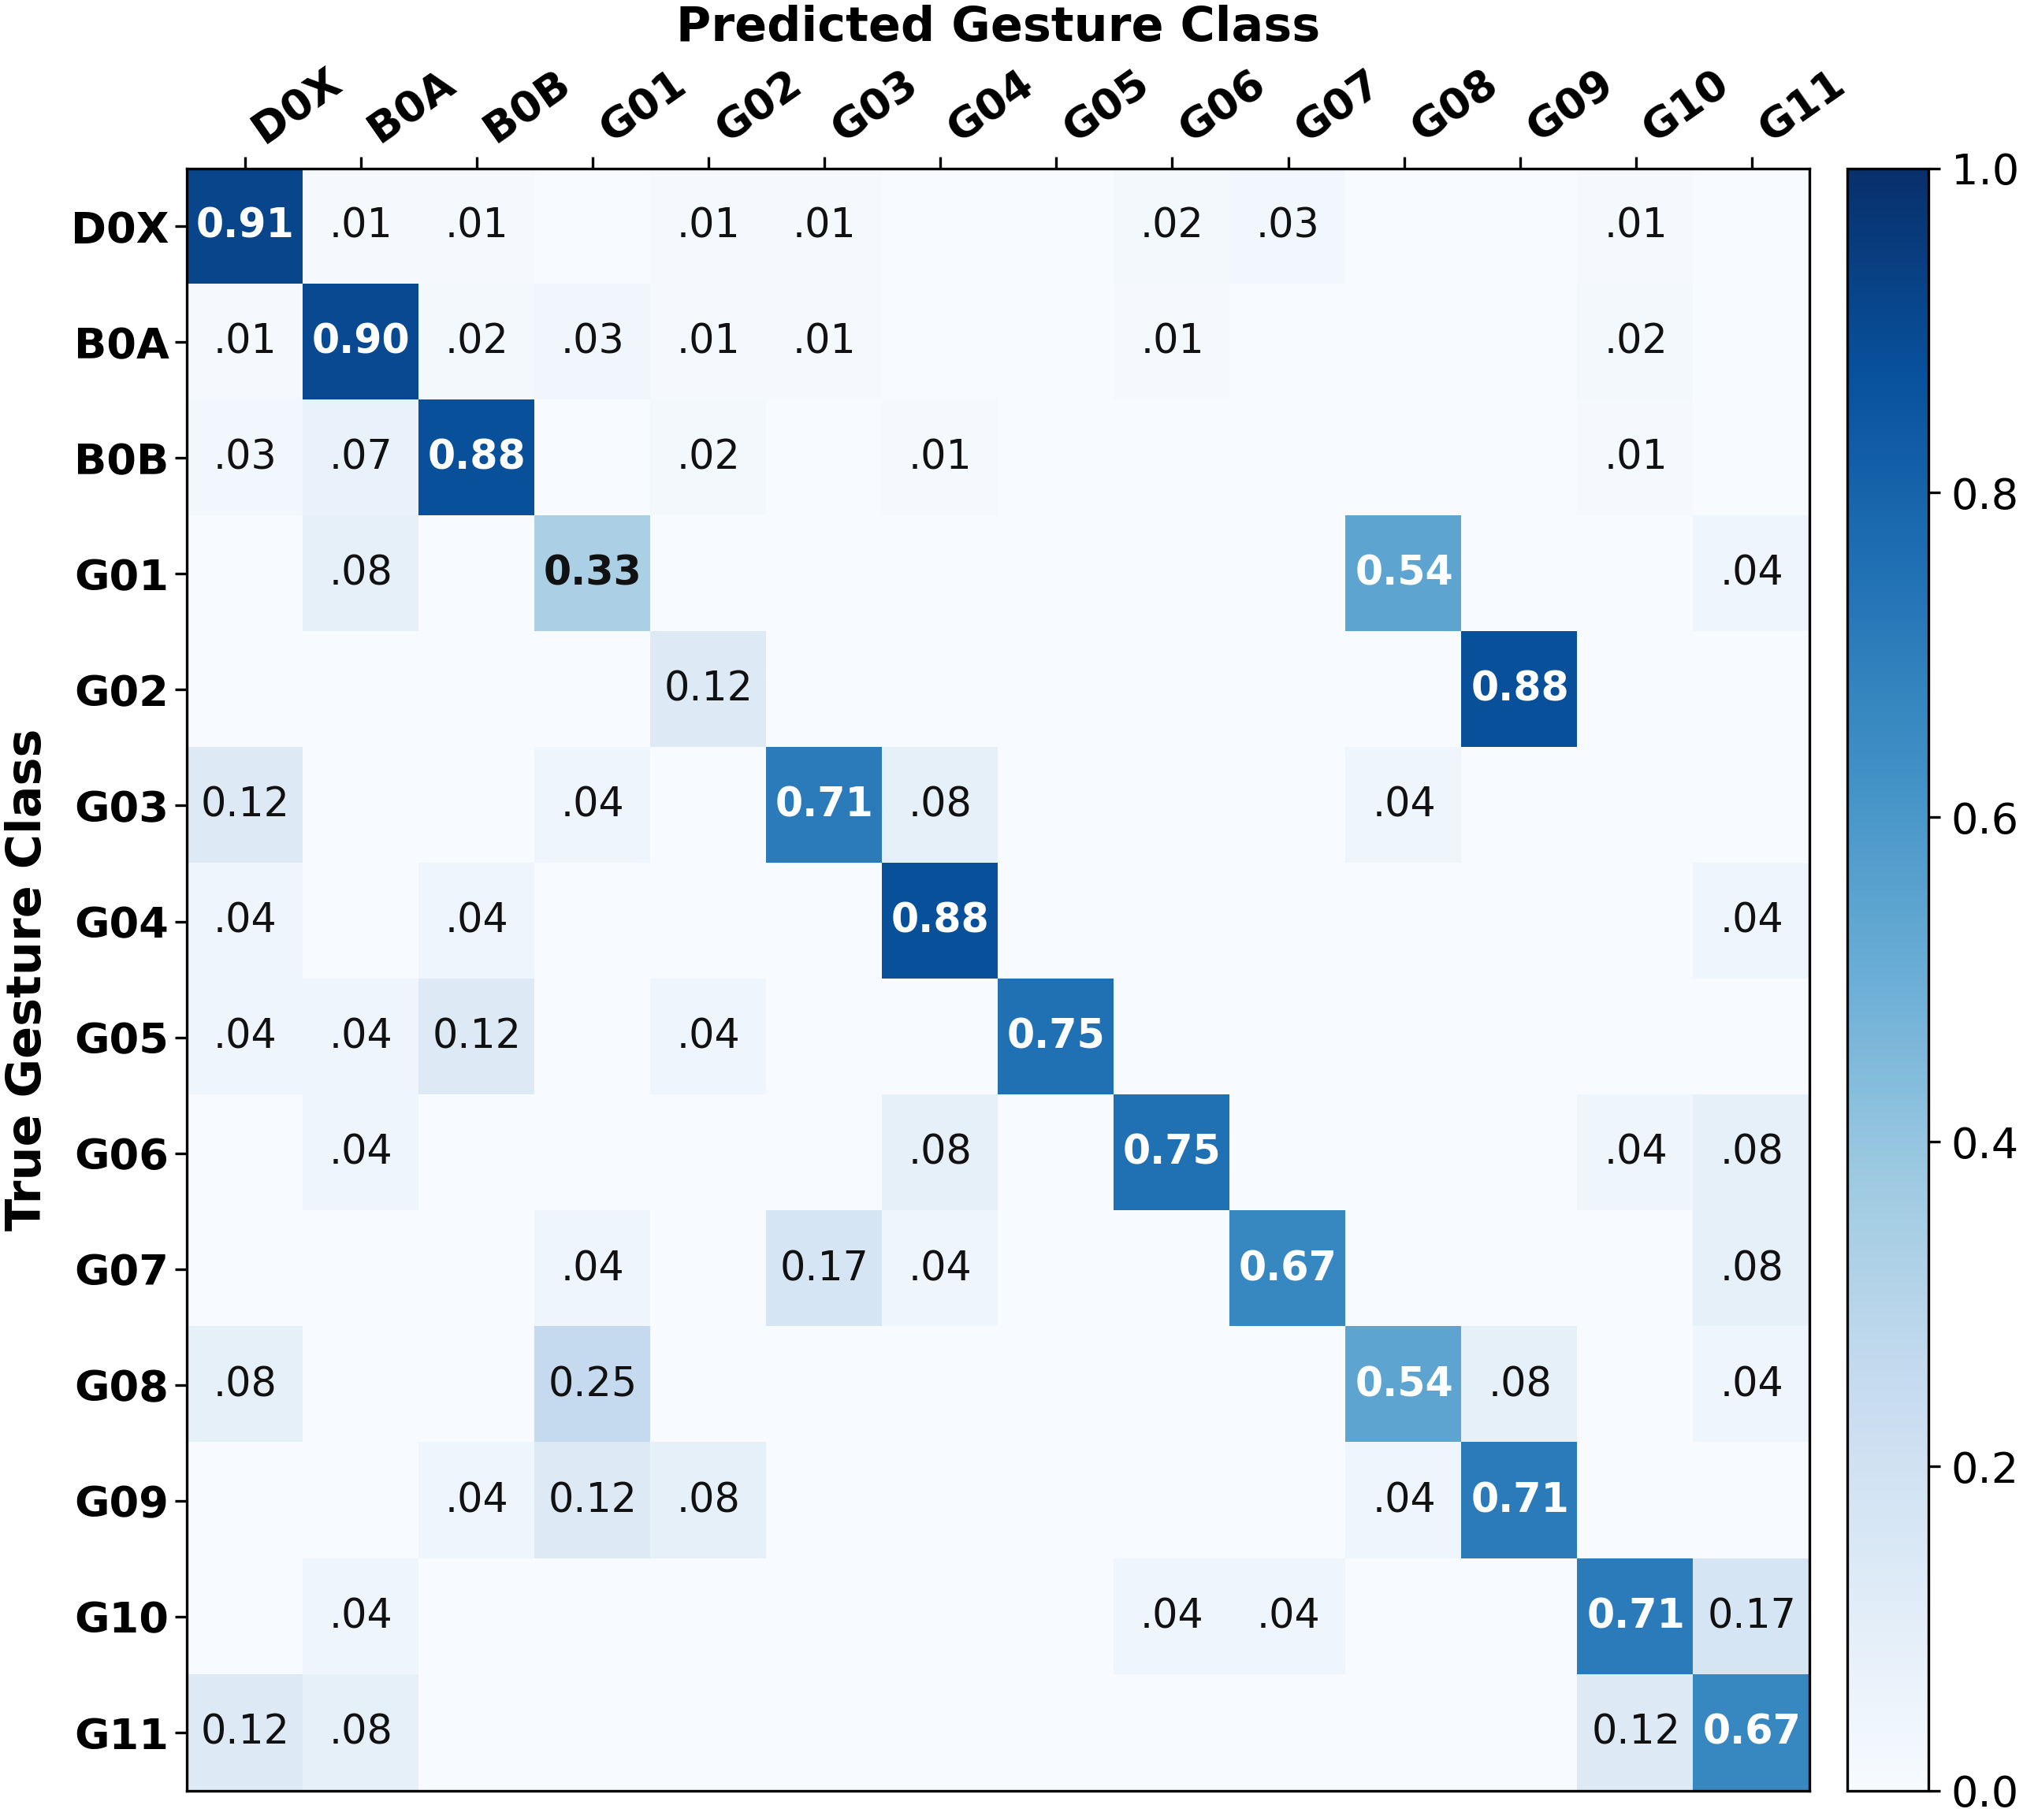
\includegraphics[width=\linewidth,height=6.30cm,keepaspectratio]{ipn_cm_fill.png}\par
    \end{column}
    \begin{column}{0.32\textwidth}
      \begin{tcolorbox}[titlepanel,title=Nhóm chính xác cao]
        {\fontsize{7.0}{8.1}\selectfont
        \begin{itemize}\tightitems
          \item \textbf{D0X, B0A, B0B:} Cử chỉ tĩnh đạt \textbf{87.5\% -- 91.5\%}.
          \item \textbf{G04--G06:} Vuốt ném đạt \textbf{75.0\% -- 87.5\%} (G05 Precision 100\%).
          \item \textbf{G10, G11:} Zoom đạt \textbf{66.7\% -- 70.8\%}.
        \end{itemize}}
      \end{tcolorbox}
      \vspace{0.08cm}
      \begin{tcolorbox}[keypanel]
        \heading{Cặp nhầm lẫn chính}
        {\fontsize{6.8}{7.9}\selectfont
        \begin{itemize}\tightitems
          \item \textbf{G01 $\leftrightarrow$ G08:} Click 1 ngón $\rightarrow$ Double (54.2\%).
          \item \textbf{G02 $\leftrightarrow$ G09:} Click 2 ngón $\rightarrow$ Double (87.5\%).
          \item \smallnote{Do 16-frame sampling bắt trùng pha chuyển động bấm của double click.}
        \end{itemize}}
      \end{tcolorbox}
    \end{column}
  \end{columns}
  \vfill
  \source{Ma trận nhầm lẫn chuẩn hóa theo nhãn thực tế (True labels) trên 622 đoạn video test.}
\end{frame}

\end{document}
